%!TEX root = main.tex
%%%%%%%%%%%%%%%%%%%%%%%%%%%%%%%%%%%%%%%%%%%%%%%%%%%%%%%%%%%%%%%%%%%%%%%%%%%%%%%%

\subsection{Heuristic Approach}

The heuristic approach uses isotonic regression \cite{barlow1972statistical} to deduce a video-dependent relationship between the data shown to the user and the resulting average quality level based on previously recorded playback sessions.
This gives an estimate of how much non-redundant data is necessary to reach a certain quality level.
Furthermore, it allows us to estimate the difference in term of average quality between two different amounts of data.
The advantage of the approach is that it captures the dynamics of the overall system as it is based on actual observations.

Figure \ref{fig:heuristic} illustrates the resulting relationship for one of the videos in the data-set.
The axis to the right gives the amount of Bytes shown to the user.
The axis to the left gives the resulting average playback quality.
Each (brown) dot represents one playback session.
The connected (black) dots are the isotonic regression result.

Multiple observations can be made from the figure. 
First, a specific amount of played bytes can result in different average quality levels at the end. 
This is due to the combinatorial problem which arises due to the different quality levels and bit-rate variations inside a quality level.
Second, there is a jump at \unit[20]{MBytes} from 0.7 to 1.1 average quality level.
Third, there are outliers, e.g. at \unit[27]{MBytes}, where significant more data does not increase the average quality level.

\begin{figure}[t]
\centering
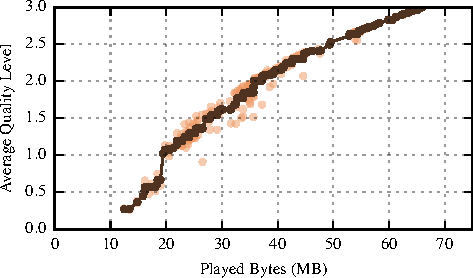
\includegraphics[width=0.9\linewidth]{figs/32_vbLLqaa9ksw.pdf}%
\caption{Isotonic regression result showing the relationship between Bytes shown to the user and resulting average playback quality for video vbLLqaa9ksw. 336 video views are used in the regression.}
\label{fig:heuristic}%
\end{figure}

